\documentclass[12pt,t]{beamer}
% \documentclass[t]{beamer}
\usepackage[utf8]{inputenc}
\usepackage[catalan]{babel}
\usepackage{verbatim}
\usepackage{hyperref}
\usepackage{amsfonts,amssymb,amsmath,amsthm, wasysym, multirow}
\usepackage{listings}
\usepackage[T1]{fontenc}        
\usepackage{pgf}
\usepackage{epsdice}
\usepackage{pgfpages}
\usepackage{tikz}
%\usetikzlibrary{arrows,shapes,plotmarks,backgrounds,trees,positioning}
%\usetikzlibrary{decorations.pathmorphing,calc,snakes}
%\usepackage{marvosym}
%
\usetheme[hideothersubsections,left]{Marburg}
\usecolortheme{sidebartab}
\useinnertheme[shadow]{rounded}
% \useoutertheme[footline=empty,subsection=true,compress]{infolines}
% \useoutertheme[footline=empty,subsection=true,compress]{miniframes}
% \usefonttheme{serif}

\setbeamertemplate{caption}[numbered]
\setbeamertemplate{navigation symbols}{}


\newcommand{\red}[1]{\textcolor{red}{#1}}
\newcommand{\green}[1]{\textcolor{green}{#1}}
\newcommand{\blue}[1]{\textcolor{blue}{#1}}
\newcommand{\gray}[1]{\textcolor{gray}{#1}}
\renewcommand{\emph}[1]{{\color{red}#1}}

\setbeamertemplate{frametitle}
{\begin{centering}
\medskip
\color{blue}
\textbf{\insertframetitle}
\medskip
\end{centering}
}
\usecolortheme{rose}
\usecolortheme{dolphin}
\mode<presentation>


\newcommand{\CC}{\mathbb{C}}
\newcommand{\RR}{\mathbb{R}}
\newcommand{\ZZ}{\mathbb{Z}}
\newcommand{\NN}{\mathbb{N}}
\newcommand{\KK}{\mathbb{K}}
\newcommand{\MM}{\mathcal{M}}
%\newcommand{\dbinom}{\displaystyle\binom}

\newcommand{\limn}{{\displaystyle \lim_{n\to\infty}}}
\renewcommand{\leq}{\leqslant}
\renewcommand{\geq}{\geqslant}
\def\tendeix{{\displaystyle\mathop{\longrightarrow}_{\scriptscriptstyle
n\to\infty}}}

\newcommand{\matriu}[1]{\left(\begin{matrix} #1 \end{matrix}\right)}

% \newcommand{\qed}{\hbox{}\nobreak\hfill\vrule width 1.4mm height 1.4mm depth 0mm
%     \par \goodbreak \smallskip}
%
% %
\theoremstyle{plain}
\newtheorem{teorema}{Teorema}
\newtheorem{prop}{Proposició}
\newtheorem{cor}{Coro\l.lari}
\theoremstyle{definition}
\newtheorem{exemple}{Exemple}
\newtheorem{defin}{Definició}
\newtheorem{obs}{Observació}

\newcounter{seccions}
\newcommand{\seccio}[1]{\addtocounter{seccions}{1}
\medskip\par\noindent\emph{\theseccions.
#1}\smallskip\par }

\newcommand{\EM}{\Omega}
\newcommand{\PP}{\mathcal{P}}

\title[\red{Matemàtiques III}]{}
\author[]{}
\date{}



\begin{document}
\beamertemplatedotitem

\lstset{backgroundcolor=\color{green!50}}
\lstset{breaklines=true}
\lstset{basicstyle=\ttfamily}


\begin{frame}
\vfill
\begin{center}
\gray{\LARGE ANOVA}
\end{center}
\vfill
\end{frame}



%%%%%
\part{ANOVA}

\section{Nocions bàsiques}
\begin{frame}
\frametitle{Problema bàsic}
\begin{itemize}
\item Tenim $k>2$ poblacions. Usualment són subpoblacions d'una única població, definides pels nivells de factors.
\medskip

\item Volem decidir si el valor mitjà d'un cert paràmetre és el mateix a totes aquestes poblacions o no
\medskip

\item Siguin $\mu_1,\ldots,\mu_k$ les mitjanes d'aquest paràmetre en aquestes poblacions. Volem fer el contrast:
$$
\left\{
\begin{array}{l}
H_0 : \mu_1 =\mu_2 =\cdots =\mu_k \\
H_1 : \exists i,j \mid  \mu_i \not=\mu_j
\end{array}
\right.
$$

\item Prendrem una mostra aleatòria de cada població, i a partir d'aquestes mostres ho decidirem
\end{itemize}



\end{frame}


\begin{frame}
\frametitle{ANOVA}
La tècnica que emprarem és l'\emph{Anàlisi de la Variància} (\emph{ANOVA}, de l'anglès \textsl{\red{AN}alysis \red{O}f \red{VA}riance})
\bigskip

Aquesta tècnica es pot aplicar sota diferents dissenys d'experiments:
\begin{itemize}
\item Segons quants factors empram per separar la població en subpoblacions
\medskip

\item Segons com triam els nivells dels factors
\medskip

\item Segons com escollim les mostres
\end{itemize}
\medskip

Veurem els dissenys més bàsics. En un problema concret, s'ha de decidir primer el tipus d'experiment que s'ha de realitzar.

\end{frame}



\begin{frame}
\frametitle{ANOVA}

Per comparar les mitjanes de dues poblacions,  calculàvem les mitjanes de dues mostres i les comparàvem
\medskip

Per comparar les mitjanes de $k\geq 3$ poblacions, podríem fer-ho per parelles, però són moltes: $\dbinom{k}{2}$
\medskip

I les hem de comparar totes, perquè pot passar que
$$
\mu_1\approx \mu_2, \mu_2\approx \mu_3, \mu_3\approx\mu_4\mbox{ però }
\mu_1\not\approx \mu_4
$$
\smallskip

Volem un test que ens digui en un pas si totes són iguals, o si n'hi ha de diferents (en aquest darrer cas, ja cercarem les diferents si volem)
\end{frame}


\begin{frame}
\frametitle{ANOVA}

Per comparar les mitjanes de 3 o més poblacions, ens concentram en la variabilitat de les dades per grups:
\medskip

\begin{itemize}
\item Variabilitat de les dades (respecte de la mitjana global)
\medskip

\item Variabilitat dins cada població (respecte de la mitjana dins la població)
\medskip

\item Variabilitat de les mitjanes per poblacions (respecte de la mitjana global)
\medskip
\end{itemize}

\begin{quote}
\red{Si la variabilitat total de les dades és explicada per la variabilitat de les mitjanes de les poblacions i  la ``poca variabilitat'' dins cada població, és indici que les mitjanes són diferents}
\end{quote}
\end{frame}


\begin{frame}
\frametitle{ANOVA}

\begin{center}
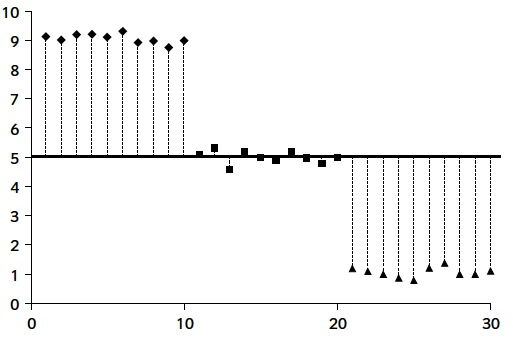
\includegraphics[width=0.8\linewidth]{FD1-1}\\
Molta variabilitat\ldots 
\end{center}
\end{frame}

\begin{frame}
\frametitle{ANOVA}

\begin{center}
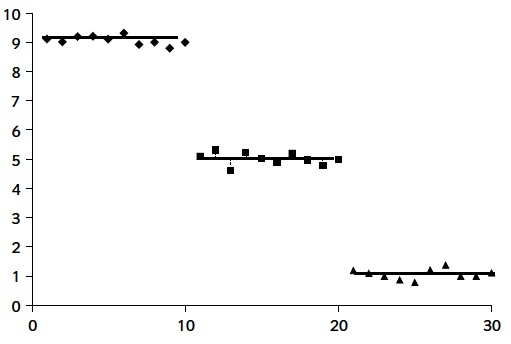
\includegraphics[width=0.8\linewidth]{FD1-2}\\
\ldots\ concentrada entorn de les mitjanes per nivells \\ \pause
\medskip

\red{Les mitjanes són (òbviament) diferents}

\end{center}
\end{frame}


\begin{frame}
\frametitle{ANOVA}

\begin{center}
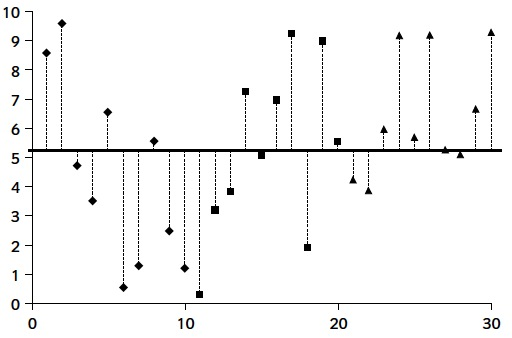
\includegraphics[width=0.8\linewidth]{FD2-1}\\
Molta variabilitat\ldots 
\end{center}
\end{frame}

\begin{frame}
\frametitle{ANOVA}

\begin{center}
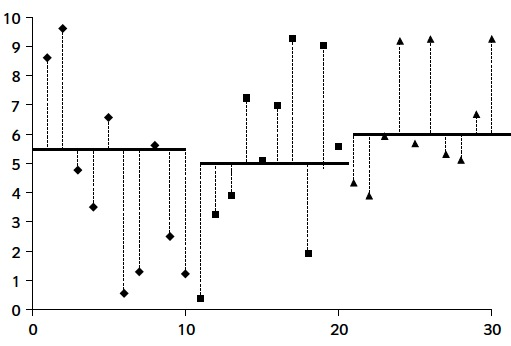
\includegraphics[width=0.8\linewidth]{FD2-2}\\
\ldots\ que no és explicada per les diferències de les mitjanes\\ \pause
\medskip

\red{Les mitjanes no semblen diferents}
\end{center}
\end{frame}

\begin{frame}
\frametitle{ANOVA}
\vspace*{1cm}

\begin{center}
\red{\Large Com quantificar-ho?}
\end{center}

\end{frame}





\section{Un factor}
\subsection{Efectes fixats}


\begin{frame}
\frametitle{Classificació simple, efectes fixats, disseny completament aleatori
}

En els experiments amb \emph{classificació simple, efectes fixats i disseny completament aleatori}:
\begin{itemize}
\item Empram un sol factor per classificar la població en subpoblacions (\emph{classificació simple})
\medskip

\item L'investigador decideix quins nivells (o \blue{tractaments}) del factor emprarà (\emph{efectes fixats})
\medskip

\item Es pren una m.a.s. de cada subpoblació,  de manera independent unes de les altres (\emph{completament aleatori})
\end{itemize}
\end{frame}


\begin{frame}
\frametitle{Exemple 1}
Es realitzà un estudi per investigar l'efecte del
CO${}_2$ sobre la taxa de creixement de {\it Pseudomonas fragi} (un corruptor d'aliments). 
Es creu que el creixement es veu afectat per la quantitat de CO${}_2$ en l'aire.
\medskip

Per contrastar-ho, en un experiment s'administrà CO${}_2$ a 5 pressions atmosfèriques
diferents a 10 cultius diferents per cada nivell, i s'anotà el canvi (en \%) de la massa ce\l.lular
al cap d'una hora

\end{frame}

\begin{frame}
\frametitle{Exemple 1: Dades obtingudes}
\begin{center}
\begin{tabular}{rrrrr}
\multicolumn{5}{c}{Pressió de CO${}_2$ (en atmosferes)}\\\hline
$0.0$&$0.083$&$0.29$&$0.50$&$0.86$\\\hline
$62.6$&$50.9$&$45.5$&$29.5$&$24.9$\\
$59.6$&$44.3$&$41.1$&$22.8$&$17.2$\\
$64.5$&$47.5$&$29.8$&$19.2$&$7.8$\\
$59.3$&$49.5$&$38.3$&$20.6$&$10.5$\\
$58.6$&$48.5$&$40.2$&$29.2$&$17.8$\\
$64.6$&$50.4$&$38.5$&$24.1$&$22.1$\\
$50.9$&$35.2$&$30.2$&$22.6$&$22.6$\\
$56.2$&$49.9$&$27.0$&$32.7$&$16.8$\\
$52.3$&$42.6$&$40.0$&$24.4$&$15.9$\\
$62.8$&$41.6$&$33.9$&$29.6$&$8.8$\\
\end{tabular}
\end{center}
\end{frame}





\begin{frame}
\frametitle{Exemple 2}
Disposam de quatre tractaments genètics diferents per corregir un cert gen defectuós responsable d'una malaltia. Els investigadors creuen que els quatre tractaments tenen una eficàcia similar.
\medskip

Per contrastar-ho, prenen 20 malalts diferents a l'atzar, els reparteixen aleatòriament en 4 grups de 5 malalts, i assignen de forma aleatòria un dels quatre tractaments a cada grup
\medskip

Després d'aplicar el tractament, mesuren l'expressió del gen defectuós sota estudi



\end{frame}

\begin{frame}
\frametitle{Exemple 2: Dades obtingudes}
\begin{center}
\begin{tabular}{llll}
\multicolumn{4}{c}{Tractament}\\
\hline
A & B & C & D \\
\hline
96 & 93 & 70 &  78 \\
99 & 90 & 90 & 87 \\
100 & 75 & 84 & 57 \\
104 & 80 & 76 & 66  \\
84 & 90 & 78 & 76
\end{tabular}
\end{center}

\end{frame}

\begin{frame}
\frametitle{Tipus d'experiments}

Són experiments amb classificació simple, efectes fixats i disseny completament aleatori
\begin{itemize}
\item Empram un sol factor (pressió, tractament)
\medskip

\item Decidim quins nivells empram (els que hem decidit emprar)
\medskip

\item Hem pres una m.a.s. de cada nivell del factor, i de manera independent
\end{itemize}
\end{frame}

\begin{frame}
\frametitle{Exemple 1}
Emmagatzemaré les dades  en  un \textsl{dataframe} amb dues variables:
\begin{itemize}
\item \texttt{Inc}: increment massa ce\l.lular (en \%)
\item \texttt{Pre}: Nivell de pressió, com a factor
\end{itemize}

{\footnotesize \begin{center}
\begin{tabular}{rrrrr}
\multicolumn{5}{c}{Pressió de CO${}_2$ (en atmosferes)}\\\hline
$0.0$&$0.083$&$0.29$&$0.50$&$0.86$\\\hline
$62.6$&$50.9$&$45.5$&$29.5$&$24.9$\\
$59.6$&$44.3$&$41.1$&$22.8$&$17.2$\\
$64.5$&$47.5$&$29.8$&$19.2$&$7.8$\\
$59.3$&$49.5$&$38.3$&$20.6$&$10.5$\\
$58.6$&$48.5$&$40.2$&$29.2$&$17.8$\\
$64.6$&$50.4$&$38.5$&$24.1$&$22.1$\\
$50.9$&$35.2$&$30.2$&$22.6$&$22.6$\\
$56.2$&$49.9$&$27.0$&$32.7$&$16.8$\\
$52.3$&$42.6$&$40.0$&$24.4$&$15.9$\\
$62.8$&$41.6$&$33.9$&$29.6$&$8.8$\\
\end{tabular}
\end{center}
}\end{frame}


\begin{frame}[fragile]
\frametitle{Exemple 1}
Emmagatzemaré les dades  en  un \textsl{dataframe} amb dues variables:
\begin{itemize}
\item \texttt{Inc}: increment massa ce\l.lular (en \%)
\item \texttt{Pre}: Nivell de pressió, com a factor
\end{itemize}
{\small \begin{verbatim}
> Inc=c(62.6,50.9,45.5,
 29.5,24.9,59.6,44.3, 41.1,22.8,
 17.2,64.5,47.5,29.8,19.2,
 7.8,59.3, 49.5,38.3,20.6,10.5,58.6,48.5,40.2,
 29.2,17.8, 64.6,50.4,38.5,24.1,22.1,50.9,35.2,
 30.2,22.6, 22.6,56.2,49.9,27.0,32.7,16.8,52.3,
 42.6,40.0, 24.4,15.9,62.8,41.6,33.9,29.6,8.8)
> Pre=rep(c("0.0","0.083","0.29","0.50","0.86"),
 times=10)
\end{verbatim}
}
\end{frame}

\begin{frame}[fragile]
\frametitle{Exemple 1}

{\small \begin{verbatim}
> CO2=data.frame(Inc,Pre)
> str(CO2)
'data.frame':	50 obs. of  2 variables:
 $ Inc: num  62.6 50.9 45.5 29.5 24.9 59.6 44.3 
   41.1 22.8 17.2 ...
 $ Pre: Factor w/ 5 levels "0.0","0.083",..: 1 2 3 
   4 5 1 2 3 4 5 ...
> head(CO2,4)
   Inc   Pre
1 62.6   0.0
2 50.9 0.083
3 45.5  0.29
4 29.5  0.50
\end{verbatim}
}

\end{frame}


\begin{frame}
\frametitle{Exemple 1: Donau una ullada a les dades}
\vspace*{-5ex}

\begin{center}
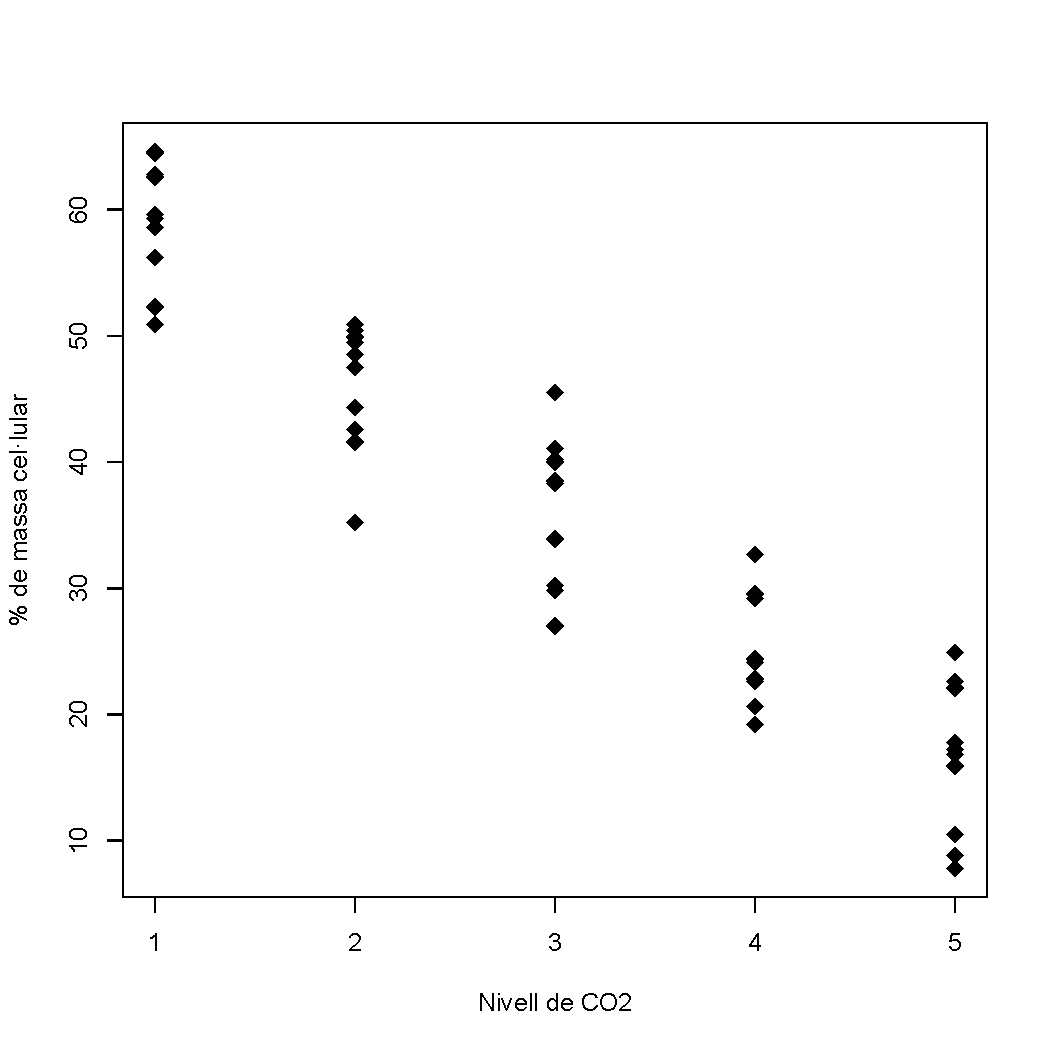
\includegraphics[width=0.8\linewidth]{nivellCO2b.pdf}
\end{center}
\end{frame}


\begin{frame}
\frametitle{Exemple 1: Donau una ullada a les dades}
\vspace*{-8ex}

\begin{center}
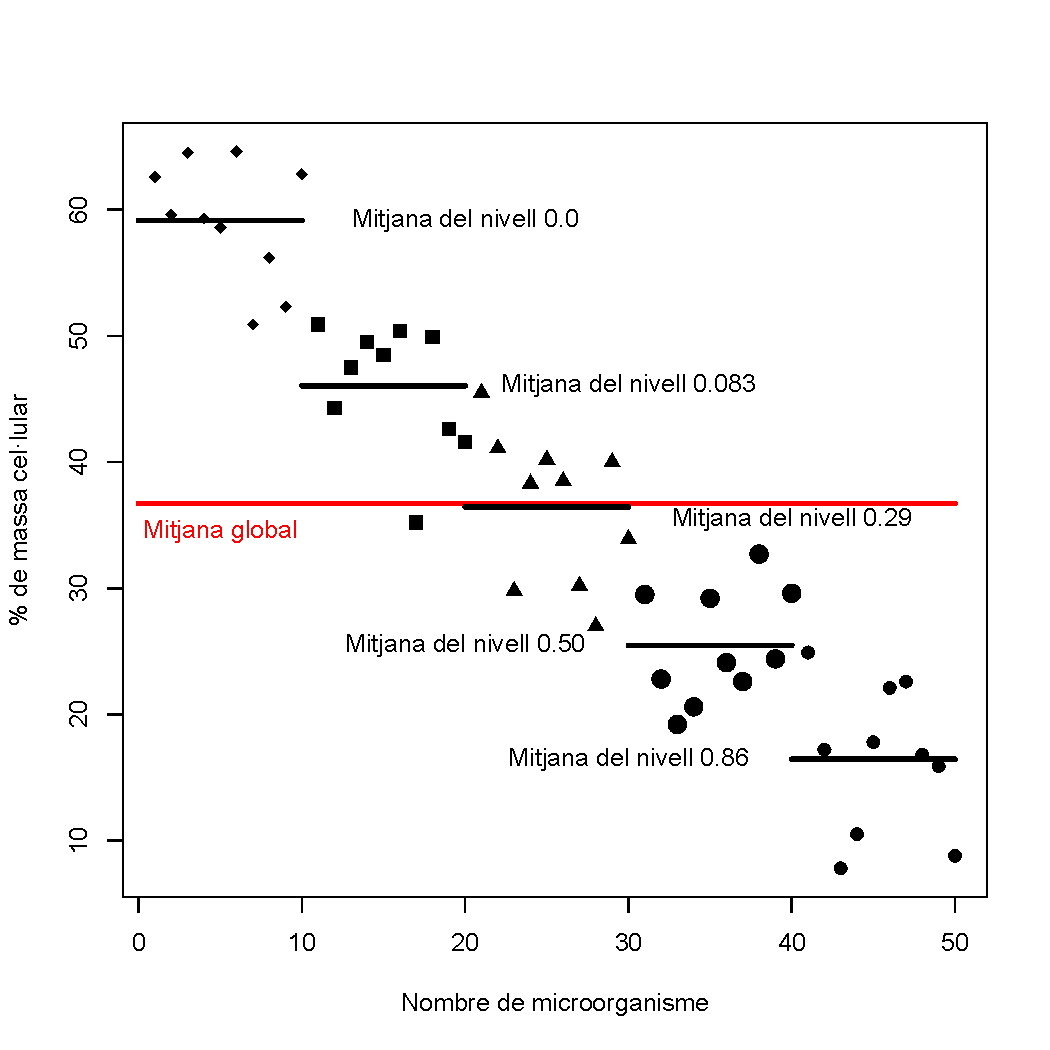
\includegraphics[width=0.8\linewidth]{varCO2-1.pdf}\\
Variabilitat de les dades
\end{center}

\end{frame}


\begin{frame}
\frametitle{Exemple 2}
\vspace*{2cm}

Vosaltres l'anireu fent a mà  {\Large \smiley}

\end{frame}


\begin{frame}
\frametitle{Notacions}

Suposarem les dades donades amb l'estructura següent
\begin{center}
\begin{tabular}{cccc}
\multicolumn{4}{c}{Nivell del factor}\\\hline
$1$&$2$&$\cdots$&$k$\\\hline
$X_{11}$&$X_{21}$&$\cdots$&$X_{k1}$\\
$X_{12}$&$X_{22}$&$\cdots$&$X_{k2}$\\
$\cdots$&$\cdots$&$\cdots$&$\cdots$\\
$X_{1n_1}$&$X_{2n_2}$&$\cdots$&$X_{kn_k}$\\\hline
\end{tabular}
\end{center}
on 
\begin{itemize}
\item \emph{$n_i$} és la mida de la mostra del nivell $i$
\medskip

\item \red{$X_{ij}$} és el valor de la característica sota estudi a l'individu $j$ del nivell $i$
\end{itemize}
\medskip

\red{\bf ALERTA!} Notacions diferents que a les matrius. A $X_{\red{i}\blue{j}}$, \red{$i$} indica la \red{columna} i \blue{$j$} la \blue{filera}

\end{frame}

\begin{frame}
\frametitle{Estadístics}
\begin{itemize}
\item Suma total de les dades del nivell $i$-èsim: $$\red{T_{i\bullet}}
=\sum_{j=1}^{n_i} X_{ij}$$
\item Mitjana mostral per al nivell $i$-èsim: $$\red{\overline{X}_{i\bullet}} =
\frac{T_{i\bullet}}{n_i}$$
\item Suma total de les dades: $$\red{T_{\bullet\bullet}}=\sum_{i=1}^k
\sum_{j=1}^{n_i} X_{ij} =\sum_{i=1}^k T_{i\bullet}$$
\item Mitjana mostral de totes les dades: $$\red{\overline{X}_{\bullet\bullet}}
=\frac{T_{\bullet\bullet}}{N}, \qquad \mbox{on } N=n_1+\cdots + n_k$$
\end{itemize}
\end{frame}


\begin{frame}[fragile]
\frametitle{Exemple 1}

\begin{verbatim}
> str(CO2)
'data.frame':	50 obs. of  2 variables:
 $ Inc: num  62.6 50.9 45.5 29.5 24.9 59.6 
   44.3 41.1 22.8 17.2 ...
 $ Pre: Factor w/ 5 levels "0.0","0.083",..: 
   1 2 3 4 5 1 2 3 4 5 ...
\end{verbatim}

\end{frame}


\begin{frame}[fragile]
\frametitle{Exemple 1}
\vspace*{-2ex}

Calculam els estadístics:\medskip

\blue{$\mathbf \bullet$} Sumes per nivells:

\begin{verbatim}
> sumes.nivells=
   aggregate(Inc~Pre,data=CO2,sum)
> sumes.nivells
    Pre   Inc
1   0.0 591.4
2 0.083 460.4
3  0.29 364.5
4  0.50 254.7
5  0.86 164.4
\end{verbatim}
\end{frame}



\begin{frame}[fragile]
\frametitle{Exemple 1}
Calculam els estadístics:\medskip

\blue{$\mathbf \bullet$} Mitjanes per nivells:

\begin{verbatim}
> mitjanes.nivells=
   aggregate(Inc~Pre,data=CO2,mean)
> mitjanes.nivells
    Pre   Inc
1   0.0 59.14
2 0.083 46.04
3  0.29 36.45
4  0.50 25.47
5  0.86 16.44
\end{verbatim}

\end{frame}



\begin{frame}[fragile]
\frametitle{Exemple 1}
Calculam els estadístics:\medskip

\blue{$\mathbf \bullet$} Suma total de les dades:

\begin{verbatim}
> suma.total=sum(CO2$Inc)
> suma.total
[1] 1835.4
\end{verbatim}\medskip

\blue{$\mathbf \bullet$} Mitjana de totes les dades:

\begin{verbatim}
> mitjana.total=mean(CO2$Inc)
> mitjana.total
[1] 36.708
\end{verbatim}

\end{frame}
\begin{frame}
\frametitle{Exemple 2}
Calculau els estadístics:
\begin{itemize}
\item Sumes totals de les dades per nivells:
\begin{center}
\begin{tabular}{c|c|c|c}
\quad${T_{1\bullet}}$\quad{} & \quad${T_{2\bullet}}$\quad{} & \quad${T_{3\bullet}}$\quad{} & \quad${T_{4\bullet}}$\quad{} \\
\hline
 &
 &
 & 
\end{tabular}
\end{center}
\medskip

\item Mitjanes mostrals per nivells:
\begin{center}
\begin{tabular}{c|c|c|c}
\quad${\overline{X}_{1\bullet}}$\quad{} & \quad${\overline{X}_{2\bullet}}$\quad{} & \quad${\overline{X}_{3\bullet}}$\quad{} & \quad${\overline{X}_{4\bullet}}$\quad{} \\
\hline
&
&
&
\end{tabular}
\end{center}
\medskip

\item Suma total de les dades: $T_{\bullet\bullet}=$
\medskip



\item Mitjana mostral de totes les dades: $\overline{X}_{\bullet\bullet}=$

\end{itemize}

\end{frame}



\begin{frame}
\frametitle{Exemple 2}
Calculau els estadístics:
\begin{itemize}
\item Sumes totals de les dades per nivells:
\begin{center}
\begin{tabular}{c|c|c|c}
\quad${T_{1\bullet}}$\quad{} & \quad${T_{2\bullet}}$\quad{} & \quad${T_{3\bullet}}$\quad{} & \quad${T_{4\bullet}}$\quad{} \\
\hline
483 &
428 &
398 &
364
\end{tabular}
\end{center}
\medskip

\item Mitjanes mostrals per nivells:
\begin{center}
\begin{tabular}{c|c|c|c}
\quad${\overline{X}_{1\bullet}}$\quad{} & \quad${\overline{X}_{2\bullet}}$\quad{} & \quad${\overline{X}_{3\bullet}}$\quad{} & \quad${\overline{X}_{4\bullet}}$\quad{} \\
\hline
$96.6$ &
$85.6$ &
$79.6$ &
$72.8$ 
\end{tabular}
\end{center}
\medskip

\item Suma total de les dades: $T_{\bullet\bullet}=1673$
\medskip



\item Mitjana mostral de totes les dades: $\overline{X}_{\bullet\bullet}=83.65$

\end{itemize}

\end{frame}


\begin{frame}
\frametitle{El model}
Els paràmetres que intervindran en el contrast són:
\begin{itemize}
\item \red{$\mu$}: mitjana poblacional  del conjunt de la població  (ignorant els nivells)
\medskip

\item \red{$\mu_i$}: mitjana poblacional dins el nivell $i$-èsim,
$i=1,\ldots,k$
\medskip
\end{itemize}
\medskip

Els estimadors dels paràmetres són els següents:
\begin{itemize}
\item \red{De $\mu$}: $\overline{X}_{\bullet\bullet}$
\medskip

\item \red{De cada $\mu_i$}: $\overline{X}_{i\bullet}$
\end{itemize}

\end{frame}


\begin{frame}
\frametitle{El model}

Les suposicions del model són:
\begin{itemize}
\item Les $k$ mostres són m.a.s. independents
extretes de $k$ poblacions específiques amb mitjanes $\mu_1,\ldots,\mu_k$
\medskip

\item Cadascuna de les $k$ poblacions segueix una llei normal
\medskip

\item Totes aquestes poblacions tenen la mateixa variància $\sigma^2$
\end{itemize}
\end{frame}


\begin{frame}
\frametitle{El model}

\emph{Expressió matemàtica} del model a estudiar en aquest cas:
$$
X_{ij} -\mu=(X_{ij} -\mu_i)+(\mu_i - \mu),\ i=1,\ldots,k,\ j=1,\ldots,n_i,
$$
on
\begin{itemize}
\item \red{$X_{ij}$}: valor del $j$-èsim individu dins del nivell $i$-èsim
\medskip

\item \red{$X_{ij}-\mu$}: desviació de l'individu respecte de la mitjana global
\medskip

\item \red{$X_{ij}-\mu_i$}: desviació de l'individu respecte de la mitjana del seu grup 
\medskip

\item \red{$\mu_i -\mu$}: desviació de la mitjana del grup $i$-èsim respecte de la mitjana global 
\end{itemize}
\end{frame}



\begin{frame}
\frametitle{El model}

\emph{Expressió matemàtica} del model a estudiar en aquest cas:
$$
X_{ij} -\mu=(X_{ij} -\mu_i)+(\mu_i - \mu),\ i=1,\ldots,k,\ j=1,\ldots,n_i,
$$
i
\begin{itemize}
\item \red{$X_{ij}-\overline{X}_{\bullet\bullet}$} estima $X_{ij} - \mu$
\medskip


\item \red{$X_{ij}-\overline{X}_{i\bullet}$} estima $X_{ij} -\mu_i$
\medskip



\item \red{$\overline{X}_{i\bullet}-\overline{X}_{\bullet\bullet}$} estima $\mu_i - \mu$
\end{itemize}
\end{frame}

%%%%%%%%%
\begin{frame}
\frametitle{Identitat de la suma de quadrats}
\begin{teorema}
{\small 
$\displaystyle \sum_{i=1}^k\sum_{j=1}^{n_i} (X_{ij}-\overline{X}_{\bullet\bullet})^2 =
\sum_{i=1}^k n_i (\overline{X}_{i\bullet}-\overline{X}_{\bullet\bullet})^2 +
\sum_{i=1}^k\sum_{j=1}^{n_i} (X_{ij}-\overline{X}_{i\bullet})^2$
}
\end{teorema}
\begin{itemize}
\item $\red{SS_{Total}}=\sum\limits_{i=1}^k\sum\limits_{j=1}^{n_i} (X_{ij}-\overline{X}_{\bullet\bullet})^2$   (\red{Suma Total de Quadrats})

\item $\red{SS_{Tr}}=\sum\limits_{i=1}^k n_i
(\overline{X}_{i\bullet}-\overline{X}_{\bullet\bullet})^2$ (\red{Suma de Quadrats dels Tractaments}) 

\item $\red{SS_E}=\sum\limits_{i=1}^k\sum\limits_{j=1}^{n_i} (X_{ij}-\overline{X}_{i\bullet})^2$
(\red{Suma de Quadrats dels Residus} o \red{Errors})
\end{itemize}
\end{frame}

\begin{frame}
\frametitle{Identitat de la suma de quadrats}
\begin{teorema}
$SS_{Total}=SS_{Tr}+SS_E$
\end{teorema}
\begin{itemize}
\item $\red{SS_{Total}}=\sum\limits_{i=1}^k\sum\limits_{j=1}^{n_i} (X_{ij}-\overline{X}_{\bullet\bullet})^2$   

\item $\red{SS_{Tr}}=\sum\limits_{i=1}^k n_i
(\overline{X}_{i\bullet}-\overline{X}_{\bullet\bullet})^2$  

\item $\red{SS_E}=\sum\limits_{i=1}^k\sum\limits_{j=1}^{n_i} (X_{ij}-\overline{X}_{i\bullet})^2$
\end{itemize}
\end{frame}






\begin{frame}
\frametitle{Identitat de la suma de quadrats}
\begin{teorema}
$SS_{Total}=SS_{Tr}+SS_E$
\end{teorema}

A mà, s'empren les fórmules, equivalents, següents:
\begin{itemize}
\item $\displaystyle \red{SS_{Total}}=\sum_{i=1}^k\sum_{j=1}^{n_i} X_{ij}^2 - \frac{T_{\bullet\bullet}^2}{N}$

\item $\displaystyle \red{SS_{Tr}}=\sum_{i=1}^k \frac{T_{i\bullet}^2}{n_i} -\frac{T_{\bullet\bullet}^2}{N}$  


\item $\red{SS_E}=SS_{Total}-SS_{Tr}$
\end{itemize}
\medskip

Usualment escriurem, per abreviar,
$$
\red{T^{(2)}_{\bullet\bullet}}=\sum\limits_{i=1}^k\sum\limits_{j=1}^{n_i} X_{ij}^2
$$
\end{frame}





\begin{frame}[fragile]
\frametitle{Exemple 1}
\begin{itemize}
\item $SS_{Total}=\sum\limits_{i=1}^k\sum\limits_{j=1}^{n_i} (X_{ij}-\overline{X}_{\bullet\bullet})^2=\sum\limits_{i=1}^k\sum\limits_{j=1}^{n_i} X_{ij}^2 - \dfrac{T_{\bullet\bullet}^2}{N}$
\begin{verbatim}
> SSTotal1=sum((CO2$Inc-mitjana.total)^2)
> SSTotal1
[1] 12522.36
> SSTotal=sum(CO2$Inc^2)-suma.total^2/50
> SSTotal
[1] 12522.36
\end{verbatim}
\end{itemize}
\end{frame}





\begin{frame}[fragile]
\frametitle{Exemple 1}
\begin{itemize}
\item $SS_{Tr}=\sum\limits_{i=1}^k n_i
(\overline{X}_{i\bullet}-\overline{X}_{\bullet\bullet})^2=\sum\limits_{i=1}^k \dfrac{T_{i\bullet}^2}{n_i} -\dfrac{T_{\bullet\bullet}^2}{N}$
\medskip

\hspace*{-3ex}\begin{minipage}{\textwidth}
\begin{verbatim}
> SSTr1=sum(table(CO2$Pre)*
 (mitjanes.nivells[,2]-mitjana.total)^2)
> SSTr1
[1] 11274.32
> SSTr=sum(sumes.nivells[,2]^2/table(CO2$Pre))
   -(suma.total^2)/50
> SSTr 
[1] 11274.32
\end{verbatim}
\end{minipage}
\end{itemize}
\end{frame}





\begin{frame}[fragile]
\frametitle{Exemple 1}
\begin{itemize}
\item  $SS_E=\sum\limits_{i=1}^k\sum\limits_{j=1}^{n_i} (X_{ij}-\overline{X}_{i\bullet})^2=SS_{Total}-SS_{Tr}$
\medskip

\hspace*{-3ex}\begin{minipage}{\textwidth}
\begin{verbatim}
> SSE1=sum((CO2$Inc-mitjanes.nivells[,2])^2)
> SSE1
[1] 1248.038
> SSE=SSTotal-SSTr
> SSE
[1] 1248.038
\end{verbatim}
\end{minipage}
\end{itemize}
\end{frame}


\begin{frame}
\frametitle{Exemple 2}
$n_i=5$, $i=1,\ldots,4$, $N=20$
\medskip

\begin{center}
\begin{tabular}{c|c|c|c|c|c}
\ ${T_{1\bullet}}$\ {} & \ ${T_{2\bullet}}$\ {} & \ ${T_{3\bullet}}$\ {} & \ ${T_{4\bullet}}$\ {} & \ $T_{\bullet\bullet}$\ {} & \ $T_{\bullet\bullet}^{(2)}$\ {} \\
\hline
483 &
428 &
398 &
364 &
1673 &
142713
\end{tabular}
\end{center}
\medskip

\only<1>{\begin{itemize}
\item $SS_{Total}\displaystyle=T_{\bullet\bullet}^{(2)} - \frac{T_{\bullet\bullet}^2}{N}=$
\medskip

\item $SS_{Tr}\displaystyle=\sum_{i=1}^k \frac{T_{i\bullet}^2}{n_i} -\frac{T_{\bullet\bullet}^2}{N}=$
\medskip

\item  $SS_E=SS_{Total}-SS_{Tr}=$

\end{itemize}}
\only<2>{\begin{itemize}
\item $SS_{Total}\displaystyle=T_{\bullet\bullet}^{(2)} - \frac{T_{\bullet\bullet}^2}{N}=2766.55$
\medskip

\item $SS_{Tr}\displaystyle=\sum_{i=1}^k \frac{T_{i\bullet}^2}{n_i} -\frac{T_{\bullet\bullet}^2}{N}=1528.15$
\medskip

\item  $SS_E=SS_{Total}-SS_{Tr}=1238.4$

\end{itemize}}
\end{frame}




%%%%%%%%%%

\begin{frame}
\frametitle{Estadístics del contrast}

Emprarem els estadístics següents:
\begin{itemize}
\item \emph{Quadrat mitjà dels tractaments}:
$$
\red{MS_{Tr}}=\frac{SS_{Tr}}{k-1}
$$
\item \emph{Quadrat mitjà residual}:
$$
\red{MS_E}=\frac{SS_E}{N-k}
$$
\end{itemize}
\end{frame}


\begin{frame}
\frametitle{Estadístics del contrast}

Aquests estadístics són variables aleatòries, i es té que
\begin{itemize}
\item $E(MS_{Tr})=\displaystyle\sigma^2 + \sum_{i=1}^k \frac{n_i (\mu_i
-\mu)^2}{k-1}$
\medskip

\item $E(MS_E)=\sigma^2$
\end{itemize}
\bigskip

En particular, \red{es pot usar $MS_E$ per estimar la
variància comuna $\sigma^2$}
\pause\medskip


Si $H_0:\mu_1=\cdots=\mu_k=\mu$ és certa,
$$
\sum_{i=1}^k \frac{n_i (\mu_i -\mu)^2}{k-1}=0,
$$
i si $H_0$ no és certa, aquesta quantitat és $>0$

\end{frame}


\begin{frame}
\frametitle{Estadístics del contrast}

Per tant
\medskip

\begin{itemize}
\item si $H_0$ és certa, $E(MS_E)=E(MS_{Tr})$ i hauríem d'esperar que aquests dos estadístics  tinguessin valors propers, és a dir
$$
\frac{MS_{Tr}}{MS_E}\approx 1
$$
\item si $H_0$ és falsa, $E(MS_E)<E(MS_{Tr})$ i hauríem d'esperar que 
$$
\frac{MS_{Tr}}{MS_E}> 1
$$
\end{itemize}
\end{frame}


\begin{frame}
\frametitle{Estadístics del contrast}

Considerarem com a \emph{estadístic de contrast} el quocient 
$$
\red{F=\frac{MS_{Tr}}{MS_E}}
$$
Si $H_0$ és certa:
\medskip

\begin{itemize}
\item la seva distribució és $F_{k-1,N-k}$ (F de Fisher 
amb $k-1$ i $N-k$ graus de llibertat)
\medskip

\item el seu valor serà proper a $1$
\end{itemize}
\medskip

Per tant, rebutjarem la hipòtesi nu\l.la si $F$ és prou més gran que 1



\end{frame}

\begin{frame}
\frametitle{Contrast ANOVA}
\begin{itemize}
\item Calculam les sumes de quadrats 
$$
SS_{Total}, SS_{Tr}, SS_E
$$

\item Calculam 
$$
\hspace*{-5ex} MS_{Tr}=\frac{SS_{Tr}}{k-1},\
MS_E=\frac{SS_E}{N-k},\ F=\frac{MS_{Tr}}{MS_E}
$$

\item Calculam el p-valor
$$
P(F_{k-1,N-k}\geq F)
$$

\item Si el p-valor és més petit que el nivell de significació $\alpha$  rebutjam $H_0$ i concloem que no totes les mitjanes són iguals. En cas contrari, acceptam $H_0$.
\end{itemize}
\end{frame}

\begin{frame}[fragile]
\frametitle{Exemple 1}
\begin{itemize}
\item Ja sabem que $N=50$, $k=5$,   $SS_{Total}=12522.36$,
$SS_{Tr}=11274.32$ i $SS_E=1248.038$.
\medskip

\item Els quadrats mitjans són:
\begin{verbatim}
> N=50; k=5
> MSTr=SSTr/(k-1); MSTr
[1] 2818.58
> MSE=SSE/(N-k); MSE
[1] 27.73418
\end{verbatim}
\medskip

\item L'estadístic de contrast $F$ val:
\begin{verbatim}
> EstF=MSTr/MSE; EstF
[1] 101.6284
\end{verbatim}
\end{itemize}
\end{frame}

\begin{frame}[fragile]
\frametitle{Exemple 1}

\begin{itemize}
\item El p-valor  $P(F_{k-1,N-k}\geq F)$ val
\begin{verbatim}
> 1-pf(101.6284,4,45)
[1] 0
\end{verbatim}
\medskip

\item Per tant,
rebutjam $H_0$ i concloem que el nivell de pressió de CO${}_2$ pot influir en
el creixement del microorganisme {\it Pseudomonas fragi}
\bigskip

\emph{Alerta!} Només concloem que no totes les mitjanes són iguals: no que totes les mitjanes són diferents. \red{No és el mateix!}

\end{itemize}
\end{frame}







\begin{frame} 
\frametitle{Exemple 2}
\begin{itemize}

\item Recordem que $k=4$,  $N=20$, 
$SS_{Tr}=1528.15$, $SS_E=1238.4$
\medskip 

\item Quadrats mitjans:
$$
MS_{Tr}=\qquad\quad, 
MS_E=\qquad\quad{}
$$

\item Estadístic de contrast
$$
F=\frac{MS_{Tr}}{MS_E}=
$$

\item p-valor 
\medskip 

\item Per tant,
\end{itemize}
\end{frame}



\begin{frame} 
\frametitle{Exemple 2}
\begin{itemize}

\item Recordem que $k=4$,  $N=20$, 
$SS_{Tr}=1528.15$, $SS_E=1238.4$
\medskip 

\item Quadrats mitjans:
$$
MS_{Tr}=509.38, 
MS_E=77.4
$$

\item Estadístic de contrast
$$
F=\frac{MS_{Tr}}{MS_E}=6.58
$$

\item p-valor  $P(F_{3,16}\geq F)=0.0042$ 
\medskip 

\item Per tant, rebutjam la hipòtesi nu\l.la: no tots els tractaments tenen la mateixa efectivitat
\end{itemize}
\end{frame}


%%%%%

\begin{frame}
\frametitle{Taula ANOVA}

El contrast ANOVA es resumeix en la taula següent:
{\footnotesize \begin{center}
\hspace*{-3ex}
\begin{tabular}{ll@{}@{}l@{}@{}l@{}l@{}l}
\hline
Origen&Graus&\hspace*{0.6ex} Sumes de&\hspace*{1ex} Quadrats&\hspace*{1ex} Estadístic de&\hspace*{1ex} p-valor\\
Variació&llibertat&\multicolumn{1}{c}{quadrats}&\hspace*{1ex} mitjans&\hspace*{1ex} contrast\\\hline
Nivell \vphantom{$\displaystyle \int$} &$k-1$&\hspace*{1ex} $SS_{Tr}$&\hspace*{1ex} $MS_{Tr}=\frac{SS_{Tr}}{k-1}$&\hspace*{1ex}$F=\frac{MS_{Tr}}{MS_E}$&\hspace*{1ex} p-valor \\[1ex]
Residu&$N-k$&\hspace*{1 ex} $SS_E$&\hspace*{1ex} $MS_E=\frac{SS_E}{N-k}$&\\\hline
\end{tabular}
\end{center}}
\medskip

\only<2>{\blue{Exemple 1}
{\footnotesize \begin{center}
\begin{tabular}{ll@{}@{}l@{}@{}l@{}l@{}l}
\hline
Origen&Graus&\hspace*{0.6ex} Sumes de&\hspace*{1ex} Quadrats&\hspace*{1ex} Estadístic de & \hspace*{1ex} p-valor\\
Variació&llibertat&\multicolumn{1}{c}{quadrats}&\hspace*{1ex} mitjans&\hspace*{1ex} contrast\\\hline
Nivell \vphantom{$\displaystyle \int$} &$4$&\hspace*{1ex} $11274.32$&\hspace*{1ex} $2818.58$&\hspace*{1ex}$101.63$ & \hspace*{1ex} 0 \\[1ex]
Residu&$45$&\hspace*{1 ex} $1248.04$&\hspace*{1ex} $27.73$&\\\hline
\end{tabular}
\end{center}}}

\only<3>{\blue{Exemple 2}
{\footnotesize \begin{center}
\begin{tabular}{ll@{}@{}l@{}@{}l@{}l@{}l}
\hline
Origen&Graus&\hspace*{0.6ex} Sumes de&\hspace*{1ex} Quadrats&\hspace*{1ex} Estadístic de & \hspace*{1ex} p-valor \\
Variació&llibertat&\multicolumn{1}{c}{quadrats}&\hspace*{1ex} mitjans&\hspace*{1ex} contrast\\\hline
Nivell \vphantom{$\displaystyle \int$} & 3 & $\hspace*{1.8ex} 1528.15$ & \hspace*{1ex} $509.38$ & \hspace*{1ex} $6.58$ & \hspace*{1ex} $0.004$  \\[1ex]
Residu& 16 & \hspace*{1ex} $1238.4$ & \hspace*{1ex} $77.4$ \\\hline
\end{tabular}
\end{center}}}

\end{frame}

\begin{frame}[fragile]
\frametitle{Amb R: Exemple 1}

Amb R el contrast ANOVA de l'Exemple 1 es pot realitzar amb
{\small \begin{verbatim}
> summary(aov(CO2$Inc~CO2$Pre))
            Df Sum Sq Mean Sq F value Pr(>F)    
CO2$Pre      4  11274  2818.6   101.6 <2e-16 ***
Residuals   45   1248    27.7                   
---
Signif. codes:0‘***’0.001‘**’0.01‘*’0.05‘.’0.1‘ ’1
\end{verbatim}
}

El valor de {\tt Pr(> F)} és el p-valor del contrast
\end{frame}



\begin{frame}[fragile]
\frametitle{Amb R: Exemple 2}

{\small \begin{verbatim}
> Expr=c(96,93,70,78,99,90,90,87,100,75,84,57,104,
   80,76,66,84,90,78,76)
> Tract=rep(c("A","B","C","D"),5)
> EG=data.frame(Expr,Tract)
> str(EG)
'data.frame':	20 obs. of  2 variables:
 $ Expr : num  96 93 70 78 99 90 90 87 100 75 ...
 $ Tract: Factor w/ 4 levels "A","B","C","D": 1 2 3 
  4 1 2 3 4 1 2 ...
 \end{verbatim}
}
\end{frame}



\begin{frame}[fragile]
\frametitle{Amb R: Exemple 2}

{\small \begin{verbatim}
> summary(aov(Expr~Tract,data=EG))
            Df Sum Sq Mean Sq F value  Pr(>F)   
EG$Tract     3   1528   509.4   6.581 0.00417 **
Residuals   16   1238    77.4                   
---
Signif. codes:0‘***’0.001‘**’0.01‘*’0.05‘.’0.1‘ ’1
 \end{verbatim}
}
\end{frame}

%%%%%%%%%%%%%%%%%%%%%%%%%

\subsection{Comparacions per parelles}
\begin{frame}
\frametitle{Comparacions per parelles}

Si hem rebutjat la hipòtesi nul·la $H_0:\mu_1=\cdots =\mu_k$, podem demanar-nos
quins són els nivells diferents
\medskip

Ho podem fer de diverses maneres, aquí en veurem tres
\end{frame}

\begin{frame}
\frametitle{Comparacions per parelles}
Es realitzen els $\displaystyle\binom{k}{2}$
contrastos
$$
\left.
\begin{array}{ll}
H_0 &: \mu_i=\mu_j \\
H_1 &: \mu_i\not=\mu_j
\end{array}
\right\}
$$
L'estadístic de cada contrast 
és:
$$
T=\frac{\overline{X}_{i\bullet} - \overline{X}_{j\bullet}}{\sqrt{MS_E\cdot (\frac{1}{n_i}
+\frac{1}{n_j})}}
$$
que segueix una distribució $t$ de Student amb $N-k$ graus de
llibertat, $t_{N-k}$
\medskip

El $p$-valor de cada contrast és $2P(t_{N-k}\geq |t_{i,j}|)$, on $t_{i,j}$ és el valor que hi pren l'estadístic
\end{frame}



\begin{frame}
\frametitle{Comparacions per parelles}
\red{Alerta!}
Si es realitzen $c$ contrastos a un nivell de significació $\alpha$, la probabilitat d'Error de Tipus I a qualcun és major que $\alpha$: de fet, és $ 1-(1-\alpha)^c$
\bigskip

Per exemple, a l'exemple del CO${}_2$, si realitzam $c=\binom{5}{2}=10$ contrastos amb nivell de significació $\alpha =0.05$, la probabilitat d'Error de Tipus I a qualcun és 
$ 1-(1-0.05)^{10} \approx 0.4$.
\bigskip

Haurem de reduir el nivell de significació de cada contrast perquè la probabilitat final d'Error de Tipus I sigui $\alpha$
\end{frame}


\begin{frame}
\frametitle{Test T de Bonferroni}
Emprarem l'aproximació $1-(1-x)^c \approx cx$ i aleshores, si volem efectuar $c$ contrastos amb nivell de significació (global) $\alpha$, els farem amb nivell de significació \red{$\alpha/c$}
\bigskip

Per exemple,  a l'exemple del CO${}_2$, si realitzam els  $10$ contrastos, per obtenir un nivell de significació global  $\alpha =0.05$, efectuam cada contrast amb nivell de significació
\red{$0.005$}
\end{frame}



\begin{frame}
\frametitle{Test T de Holm (més potent)}
\vspace*{-2ex}

\begin{enumerate}
\item Siguin $C_{1},\ldots ,C_{c}$ els contrastos i $P_{1},\ldots ,P_{c}$ els p-valors corresponents
\medskip

\item Ordenam aquests $p$-valors en ordre creixent $P_{(1)}\leq \cdots\leq P_{(c)}$ i reenumeram consistentment els contrastos $C_{(1)},\ldots, C_{(c)}$
\medskip

\item Per a cada $j=1,\ldots,c$, calculam el \emph{p-valor ajustat} $\widetilde{P}_{(j)}=(c+1-j)P_{(j)}$.
\medskip

\item Aleshores rebutjam la hipòtesi nu\l.la als contrastos $C_{(j)}$ on $\widetilde{P}_{(j)}<\alpha$
 \end{enumerate}


\end{frame}



\begin{frame}[fragile]
\frametitle{Exemple 1}
$\alpha=0.05$
\medskip


Fem els càlculs per passes
\medskip

En primer lloc cream una matriu amb fileres les parelles de nivells les mitjanes dels quals contrastarem:

 \begin{verbatim}
> pars=rbind(c(1,2),c(1,3),c(1,4),c(1,5),
   c(2,3),c(2,4),c(2,5),c(3,4),c(3,5),c(4,5))
\end{verbatim}

\end{frame}

\begin{frame}[fragile]
\frametitle{Exemple 1}

A continuació calculam els valors  de tots els estadístics de contrast
\begin{verbatim}
> est.contrast.par =
 (mitjanes.nivells[pars[,1],2]
      -mitjanes.nivells[pars[,2],2])/
  (sqrt(MSE*(1/10+1/10)))
> est.contrast.par
 [1]  5.562226  9.634116 14.296195 18.130310  
 [5] 4.071889  8.733969 12.568084 4.662080  
 [9] 8.496194  3.834115
\end{verbatim}

\end{frame}

\begin{frame}[fragile]
\frametitle{Exemple 1}
\vspace*{-2ex}

Els afegim com a columna a la matriu de parelles de nivells
\begin{verbatim}
> pars=cbind(pars,est.contrast.par)
> pars
          est.contrast.par
 [1,] 1 2         5.562226
 [2,] 1 3         9.634116
 [3,] 1 4        14.296195
 [4,] 1 5        18.130310
 [5,] 2 3         4.071889
 [6,] 2 4         8.733969
 [7,] 2 5        12.568084
 [8,] 3 4         4.662080
 [9,] 3 5         8.496194
[10,] 4 5         3.834115
\end{verbatim}

\end{frame}

\begin{frame}[fragile]
\frametitle{Exemple 1}
\vspace*{-2ex}

Calculam els $p$-valors:

\begin{verbatim}
> p.valCO2=function(x){2*(1-pt(abs(x),N-k))}
> p.vals=sapply(est.contrast.par,p.valCO2)
> p.vals
 [1] 1.387522e-06 1.649791e-12 0.000000e+00
 [4] 0.000000e+00 1.863744e-04 3.021050e-11
 [7] 2.220446e-16 2.808032e-05 6.609646e-11
[10] 3.892218e-04
\end{verbatim}

\end{frame}

\begin{frame}[fragile]
\frametitle{Exemple 1}
\vspace*{-2ex}

Ho afegim com a columna a la matriu de parelles de nivells i estadístics
\begin{verbatim}
> pars=cbind(pars,p.vals)
> pars
          est.contrast.par      p.vals
 [1,] 1 2         5.562226 1.387522e-06
 [2,] 1 3         9.634116 1.649791e-12
 [3,] 1 4        14.296195 0.000000e+00
 [4,] 1 5        18.130310 0.000000e+00
 [5,] 2 3         4.071889 1.863744e-04
 [6,] 2 4         8.733969 3.021050e-11
 [7,] 2 5        12.568084 2.220446e-16
 [8,] 3 4         4.662080 2.808032e-05
 [9,] 3 5         8.496194 6.609646e-11
[10,] 4 5         3.834115 3.892218e-04
\end{verbatim}

\end{frame}
\begin{frame}[fragile]
\frametitle{Exemple 1}
\vspace*{-2ex}

\red{\bf Bonferroni}: Quins p-valors són inferiors a 0.005?
{\small \begin{verbatim}
> pars[which(p.vals<0.005),c(1,2)]        
 [1,] 1 2
 [2,] 1 3
 [3,] 1 4
 [4,] 1 5
 [5,] 2 3
 [6,] 2 4
 [7,] 2 5
 [8,] 3 4
 [9,] 3 5
[10,] 4 5
\end{verbatim}
}

Tots. Per tant, rebutjam totes les hipòtesis nu\l.les, i concloem que els nivells tenen mitjanes diferents dues a dues

\end{frame}

\begin{frame}[fragile]
\frametitle{Exemple 1}
\vspace*{-2ex}

\red{\bf Holm}: Ordenam les fileres de \texttt{pars} ordenant els p-valors de menor a major:
{\small 
\begin{verbatim}
> pars.ord=pars[order(pars[,4]),]
> pars.ord
          est.contrast.par       p.vals
 [1,] 1 4        14.296195 0.000000e+00
 [2,] 1 5        18.130310 0.000000e+00
 [3,] 2 5        12.568084 2.220446e-16
 [4,] 1 3         9.634116 1.649791e-12
 [5,] 2 4         8.733969 3.021050e-11
 [6,] 3 5         8.496194 6.609646e-11
 [7,] 1 2         5.562226 1.387522e-06
 [8,] 3 4         4.662080 2.808032e-05
 [9,] 2 3         4.071889 1.863744e-04
[10,] 4 5         3.834115 3.892218e-04
\end{verbatim}
}
\end{frame}


\begin{frame}[fragile]
\frametitle{Exemple 1}
\vspace*{-2ex}

\red{\bf Holm}: Calculam els p-valors ajustats i els afegim com a columna a \texttt{pars.ord} 
{\footnotesize \begin{verbatim}
> p.vals.adjust=pars.ord[,4]*(10+1-1:10)
> pars.ord=cbind(pars.ord,p.vals.adjust)
> pars.ord
          est.contrast.par       p.vals p.vals.adjust
 [1,] 1 4        14.296195 0.000000e+00  0.000000e+00
 [2,] 1 5        18.130310 0.000000e+00  0.000000e+00
 [3,] 2 5        12.568084 2.220446e-16  1.776357e-15
 [4,] 1 3         9.634116 1.649791e-12  1.154854e-11
 [5,] 2 4         8.733969 3.021050e-11  1.812630e-10
 [6,] 3 5         8.496194 6.609646e-11  3.304823e-10
 [7,] 1 2         5.562226 1.387522e-06  5.550090e-06
 [8,] 3 4         4.662080 2.808032e-05  8.424096e-05
 [9,] 2 3         4.071889 1.863744e-04  3.727488e-04
[10,] 4 5         3.834115 3.892218e-04  3.892218e-04
\end{verbatim}
}
\end{frame}




\begin{frame}[fragile]
\frametitle{Exemple 1}
\vspace*{-2ex}

\red{\bf Holm}: A quins contrastos $C_{(k)}$ tenim que $\widetilde{P}_{k}\leq 0.05$?
{\small \begin{verbatim}
> pars.ord[which(pars.ord[,5]<=0.05),c(1,2)]  
 [1,] 1 4
 [2,] 1 5
 [3,] 2 5
 [4,] 1 3
 [5,] 2 4
 [6,] 3 5
 [7,] 1 2
 [8,] 3 4
 [9,] 2 3
[10,] 4 5
\end{verbatim}
}
A tots, per tant rebutjam totes les hipòtesis nu\l.les, i concloem que els nivells tenen mitjanes diferents dues a dues

\end{frame}





\begin{frame}[fragile]
\frametitle{Exemple 1}

Amb R, per calcular tots els p-valors de cop podem  fer 
{\small \begin{verbatim}
> pairwise.t.test(CO2$Inc,CO2$Pre,
 p.adjust.method="none")

Pairwise comparisons using t tests 
	with pooled SD 

data:  CO2$Inc and CO2$Pre 

      0.0     0.083   0.29    0.50   
0.083 1.4e-06 -       -       -      
0.29  1.6e-12 0.00019 -       -      
0.50  < 2e-16 3.0e-11 2.8e-05 -      
0.86  < 2e-16 2.5e-16 6.6e-11 0.00039

P value adjustment method: none 
\end{verbatim}
}


\end{frame}


\begin{frame}[fragile]
\frametitle{Exemple 1}

Si no ens volem preocupar de dividir, fem \red{\texttt{p.adjust.method="bonferroni"}} i R multiplica els p-valors obtinguts pel nombre de comparacions, i això ha de ser més petit que $\alpha$
{\small \begin{verbatim}
> pairwise.t.test(CO2$Inc,CO2$Pre,
   p.adjust.method="bonferroni")

...
      0.0     0.083   0.29    0.50   
0.083 1.4e-05 -       -       -      
0.29  1.6e-11 0.00186 -       -      
0.50  < 2e-16 3.0e-10 0.00028 -      
0.86  < 2e-16 2.5e-15 6.6e-10 0.00389

P value adjustment method: bonferroni 
\end{verbatim}
}


\end{frame}


\begin{frame}[fragile]
\frametitle{Exemple 1}

Fent \red{\texttt{p.adjust.method="holm"}} (Alerta! és el per defecte) dóna els p-valors ajustats del mètode de Holm
{\small \begin{verbatim}
> pairwise.t.test(CO2$Inc,CO2$Pre,
   p.adjust.method="holm")

...
      0.0     0.083   0.29    0.50   
0.083 5.6e-06 -       -       -      
0.29  1.2e-11 0.00037 -       -      
0.50  < 2e-16 1.8e-10 8.4e-05 -      
0.86  < 2e-16 2.0e-15 3.3e-10 0.00039

P value adjustment method: holm 
\end{verbatim}
}


\end{frame}


\begin{frame}
\frametitle{Exemple 2}

\begin{itemize}
\item $N=20$, $k=4$
\medskip

\item Mitjanes mostrals per nivells:
\begin{center}
\begin{tabular}{c|c|c|c}
\quad${\overline{X}_{1\bullet}}$\quad{} & \quad${\overline{X}_{2\bullet}}$\quad{} & \quad${\overline{X}_{3\bullet}}$\quad{} & \quad${\overline{X}_{4\bullet}}$\quad{} \\
\hline
$96.6$ &
$85.6$ &
$79.6$ &
$72.8$ 
\end{tabular}
\end{center}
\medskip

\item $MS_E=77.4$
\end{itemize}
\medskip

Decidiu quines parelles de mitjanes són diferents amb $\alpha=0.05$

\end{frame}


\begin{frame} 
\frametitle{Exemple 2}
\vspace*{-3ex}

\begin{center}
\begin{tabular}{r|r|r|r|}
& & Est. contr. & $p$-valor\\
\hline
1 & 2 & & \\
1 & 3 & & \\
1 & 4 & & \\
2 & 3 & & \\
2 &4 & & \\
3 & 4 & & \\
\end{tabular}
\end{center}

\end{frame}


\begin{frame} 
\frametitle{Exemple 2}
\vspace*{-3ex}


\begin{center}
\begin{tabular}{r|r|r|r|}
& & Est. contr. & $p$-valor\\
\hline
1 & 2 & 1.977 & 0.0655  \\
1 & 3 & 3.055 & 0.0076 \\
1 & 4 & 4.277 & 0.0006 \\
2 & 3 & 1.078 & 0.2968 \\
2 &4 & 2.3 & 0.0352 \\
3 & 4 & 1.222 & 0.2394 \\
\end{tabular}
\end{center}

\end{frame}

\begin{frame} 
\frametitle{Exemple 2}
\vspace*{-3ex}


\begin{center}
\begin{tabular}{r|r|r|r|}
& & Est. contr. & $p$-valor\\
\hline
1 & 2 & 1.977 & 0.0655  \\
1 & 3 & 3.055 & 0.0076 \\
1 & 4 & 4.277 & 0.0006 \\
2 & 3 & 1.078 & 0.2968 \\
2 &4 & 2.3 & 0.0352 \\
3 & 4 & 1.222 & 0.2394 \\
\end{tabular}
\end{center}

\red{Bonferroni}: Només les comparacions (1,3) i (1,4) davallen de $0.05/6=0.0083$, són les úniques per a les que tenim evidència que són diferents. És a dir, concloem que $\mu_A\neq \mu_C$, $\mu_A\neq \mu_D$ i que no podem afirmar que les altres siguin diferents.

\end{frame}

\begin{frame} 
\frametitle{Exemple 2}


\red{Holm}: 
\begin{center}
\begin{tabular}{r|r|r|r|r|}
& & Est. contr. & p-valor & p-valor ajustat\\
\hline
1 & 4 & 4.277 & 0.0006 & \hphantom{0.0036}\\
1 & 3 & 3.055 & 0.0076 & \\
2 &4 & 2.3 & 0.0352 &  \\
1 & 2 & 1.977 & 0.0655  &  \\
3 & 4 & 1.222 & 0.2394 & \\
2 & 3 & 1.078 & 0.2968 & \\
\end{tabular}
\end{center}

\end{frame}


\begin{frame} 
\frametitle{Exemple 2}

\red{Holm}: 
\begin{center}
\begin{tabular}{r|r|r|r|r|}
& & Est. contr. & p-valor & p-valor ajustat\\
\hline
1 & 4 & 4.277 & 0.0006 & 0.0036\\
1 & 3 & 3.055 & 0.0076 & 0.0380\\
2 &4 & 2.3 & 0.0352 & 0.1408 \\
1 & 2 & 1.977 & 0.0655  & 0.1965 \\
3 & 4 & 1.222 & 0.2394 & 0.4788\\
2 & 3 & 1.078 & 0.2968 & 0.2968\\
\end{tabular}
\end{center}

Rebutjam la hipòtesi nu\l.la a (1,4) i (1,3) i l'acceptam a tots els altres
\end{frame}


\begin{frame}[fragile]
\frametitle{Exemple 2}
\vspace*{-3ex}

\begin{verbatim}
> pairwise.t.test(EG$Expr,EG$Tract,
  p.adjust.method="bonferroni")
...
  A      B      C     
B 0.3933 -      -     
C 0.0453 1.0000 -     
D 0.0035 0.2113 1.0000

P value adjustment method: bonferroni 
\end{verbatim}
Amb l'ajustament fet, els únics que davallen de 0.05 són (A,C) i (A,D)

\end{frame}


\begin{frame}[fragile]
\frametitle{Exemple 2}
\vspace*{-3ex}

\begin{verbatim}
> pairwise.t.test(EG$Expr,EG$Tract,
  p.adjust.method="holm")
...
  A      B      C     
B 0.1966 -      -     
C 0.0378 0.4787 -     
D 0.0035 0.1409 0.4787

P value adjustment method: holm 
\end{verbatim}
Amb l'ajustament de Holm, els únics que davallen de 0.05 també són (A,C) i (A,D)

\end{frame}


%%%%%%%%%%%%%%%%%%%%%%%

\begin{frame}[fragile]
\frametitle{Contrast de Duncan}
El \emph{contrast de Duncan} és un altre mètode per veure en quins nivells hi ha
diferències
\medskip

Es realitza amb la funció \texttt{duncan.test} del paquet \texttt{agricolae}. La sintaxi és
\begin{verbatim}
duncan.test(aov,"factor",group=...)$sufix
\end{verbatim}
on
\begin{itemize}
\item \texttt{aov} és el resultat de l'ANOVA de partida
\item El \texttt{factor} és el factor de l'ANOVA
\item \texttt{group} pot ser \texttt{TRUE} o \texttt{FALSE}, presenta el resultat de forma diferent
\item El \texttt{sufix} és \texttt{group} si \texttt{group=TRUE} i \texttt{comparison} si \texttt{group=FALSE}
\end{itemize}
\end{frame}


\begin{frame}[fragile]
\frametitle{Exemple 2}
\vspace*{-3ex}

{\small 
\begin{verbatim}
> install.packages("agricolae",dep=TRUE)
> library("agricolae")
> EG.aov=aov(EG$Expr~EG$Tract)
> duncan.test(EG.aov,"EG$Tract",
  group=FALSE)$comparison
      Difference   pvalue sig.        LCL      UCL
A - B       11.0 0.065545    . -0.7955155 22.79552
A - C       17.0 0.009774   **  4.6308251 29.36917
A - D       23.8 0.000971  *** 11.0722298 36.52777
B - C        6.0 0.296877      -5.7955155 17.79552
B - D       12.8 0.042338    *  0.4308251 25.16917
C - D        6.8 0.239368      -4.9955155 18.59552
\end{verbatim}
}
Dóna uns $p$-valors: els petits permeten rebutjar la hipòtesi nu\l.la corresponent
\end{frame}


\begin{frame}[fragile]
\frametitle{Exemple 2}
\vspace*{-3ex}

{\small
\begin{verbatim}
> duncan.test(EG.aov,"EG$Tract",group=TRUE)$groups
  trt means  M
1   A  96.6  a
2   B  85.6 ab
3   C  79.6 bc
4   D  72.8  c
\end{verbatim}
}
Diu que B i A, C i B, i C i D no són significativament diferents (els altres sí)
\end{frame}


\begin{frame}[fragile]
\frametitle{Exemple 1}
\vspace*{-3ex}

{\footnotesize
\begin{verbatim}
> CO2.aov=aov(CO2$Inc~CO2$Pre)
> duncan.test(CO2.aov,"CO2$Pre",
  group=FALSE)$comparison
             Difference   pvalue sig.      LCL      UCL
0.0 - 0.083       13.10 0.000001  ***  8.35644 17.84356
0.0 - 0.29        22.69 0.000000  *** 17.70152 27.67848
0.0 - 0.50        33.67 0.000000  *** 28.52085 38.81915
0.0 - 0.86        42.70 0.000000  *** 37.43466 47.96534
0.083 - 0.29       9.59 0.000186  ***  4.84644 14.33356
0.083 - 0.50      20.57 0.000000  *** 15.58152 25.55848
0.083 - 0.86      29.60 0.000000  *** 24.45085 34.74915
0.29 - 0.50       10.98 0.000028  ***  6.23644 15.72356
0.29 - 0.86       20.01 0.000000  *** 15.02152 24.99848
0.50 - 0.86        9.03 0.000389  ***  4.28644 13.77356
\end{verbatim}
}

\end{frame}


\begin{frame}[fragile]
\frametitle{Exemple 1}
\vspace*{-3ex}

{\small
\begin{verbatim}
> duncan.test(CO2.aov,"CO2$Pre",group=TRUE)$groups
    trt means M
1 0.0   59.14 a
2 0.083 46.04 b
3 0.29  36.45 c
4 0.50  25.47 d
5 0.86  16.44 e
\end{verbatim}
}

\end{frame}

\subsection{Efectes aleatoris}

\begin{frame}
\frametitle{Efectes aleatoris}

En el model d'efectes fixats, l'experimentador tria els nivells a estudiar
\medskip

Quan el nombre de nivells és molt gran, i es vol esbrinar si els nivells del factor tenen influència en el valor mitjà del paràmetre amb el contrast
$$
\left\{
\begin{array}{l}
H_0 : \mbox{Les mitjanes de \emph{tots} els nivells són iguals} \\
H_1 : \mbox{No és veritat que\ldots}
\end{array}
\right.
$$
una possibilitat és \emph{triar una m.a.s.} de $k$ nivells, i aplicar ANOVA a aquests nivells
\medskip

És el \emph{model d'efectes aleatoris}
\end{frame}

\begin{frame}
\frametitle{Efectes aleatoris}
Les suposicions del model són:

\begin{itemize}
\item Els $k$ nivells triats formen una m.a.s. del conjunt de nivells
\smallskip

\item Les mitjanes $\mu_i$ de tots els nivells segueixen una distribució normal amb valor mitjà $\mu$ (el valor mitjà de tota la població) i desviació típica $\sigma_{Tr}$
\smallskip


\item Totes les poblacions, per a tots els nivells, segueixen lleis normals
\smallskip


\item Totes les poblacions, per a tots els nivells, tenen la mateixa variància $\sigma^2$
\smallskip


\item Les $k$ mostres són m.a.s. independents
extretes de les $k$ poblacions triades
\end{itemize}
\end{frame}

\begin{frame}
\frametitle{Efectes aleatoris}

Calculam $MS_{Tr}$ i $MS_E$ com abans. Amb les hipòtesis anteriors, en aquest cas
\begin{itemize}
\item $E(MS_{Tr})=\displaystyle\sigma^2 + \frac{N-\sum_{i=1}^k \frac{n_i^2}{N}}{k-1}\cdot \sigma_{Tr}^2$
\medskip

\item $E(MS_E)=\sigma^2$
\end{itemize}
Si $H_0$ és certa, totes les mitjanes de tots els nivells són iguals, és a dir, $\sigma_{Tr}^2=0$, i per tant 
$$
\red{F=\frac{MS_{Tr}}{MS_E}}\approx 1
$$
Aquest $F$ té distribució $F_{k-1,N-k}$ si $H_0$ és certa
\medskip

Per tant \emph{el test és el mateix que al cas d'efectes fixats}, però amb els nivells seleccionats
\end{frame}


\end{document}



\begin{frame}
\frametitle{Contrast de Duncan}
El \emph{contrast de Duncan} és un altre mètode per veure en quins nivells hi ha
diferències.

\medskip

\blue{Passos}:
\begin{enumerate}
\item[(1)] S'ordenen en forma ascendent les $k$ mitjanes mostrals
\medskip

\item[(2)] Es considera cada parell $Y$ de mitjanes mostrals i es calcula el valor absolut   $D_Y$ de  la diferència entre les dues mitjanes i el nombre $p$ de mitjanes que hi ha entre les dues (incloent-les a elles dues)
\end{enumerate}
\end{frame}


\begin{frame}
\frametitle{Contrast de Duncan}
El \emph{contrast de Duncan} és un altre mètode per veure en quins nivells hi ha
diferències
\medskip

\blue{Passos}:
\begin{enumerate}

\item[(3)] Decidim que existeix diferència entre aquests dos nivells quan 
$$
D_Y> SSR_p=r_p \sqrt{\frac{MS_E (n_i +n_j)}{2 n_i n_j}}
$$
on $n_i$ i $n_j$ són les mides dels dos nivells que comparam i $r_p$ és el \emph{menor rang significatiu} amb $N-k$ graus de llibertat, que trobareu a la corresponent  taula penjada a Campus Extens
\end{enumerate}
\end{frame}





\begin{frame}
\frametitle{Exemple 1}
Les mitjanes dels cinc nivells eren
\begin{center}
\begin{tabular}{c|c|c|c|c}
${\overline{X}_{1\bullet}}$ & ${\overline{X}_{2\bullet}}$ & ${\overline{X}_{3\bullet}}$& ${\overline{X}_{4\bullet}}$& ${\overline{X}_{5\bullet}}$\\
\hline
$59.14$ &
$46.04$ &
$36.45$ &
$25.47$ &
$16.44$
\end{tabular}
\end{center}
Ordenades de menor a major:
$$
\overline{X}_{5\bullet} < \overline{X}_{4\bullet} <
\overline{X}_{3\bullet} < \overline{X}_{2\bullet} < \overline{X}_{1\bullet}
$$
\end{frame}





\begin{frame}
\frametitle{Exemple 1}

Hem de calcular les diferències següents:
\begin{itemize}
\item $\overline{X}_{1\bullet}-\overline{X}_{5\bullet}$ ($p=5$)
\item $\overline{X}_{1\bullet}-\overline{X}_{4\bullet}$ ($p=4$)
\item $\overline{X}_{1\bullet}-\overline{X}_{3\bullet}$ ($p=3$)
\item $\overline{X}_{1\bullet}-\overline{X}_{2\bullet}$ ($p=2$)
\item $\overline{X}_{2\bullet}-\overline{X}_{5\bullet}$ ($p=4$)
\item $\overline{X}_{2\bullet}-\overline{X}_{4\bullet}$ ($p=3$)
\item $\overline{X}_{2\bullet}-\overline{X}_{3\bullet}$ ($p=2$)
\item $\overline{X}_{3\bullet}-\overline{X}_{5\bullet}$ ($p=3$)
\item $\overline{X}_{3\bullet}-\overline{X}_{4\bullet}$ ($p=2$)
\item $\overline{X}_{4\bullet}-\overline{X}_{5\bullet}$ ($p=2$)
\end{itemize}
\end{frame}

\begin{frame}
\frametitle{Exemple 1}

Tenim $n_i =10$ per a cada $i$, i per tant
$$
SSR_p=r_p \sqrt{\frac{MS_E}{10}}
$$
Calculem els valors de $SSR_p$ per a cada $p=2,3,4,5$
i amb el nivell de significació $\alpha =0.05$ (en la taula
de $r_p$ empram $40$ com a graus de llibertat de l'error ja que és el valor més
proper a $N-k=45$)
\begin{center}
\begin{tabular}{|r|r|r|r|r|}
\hline
$p$&$2$&$3$&$4$&$5$\\\hline
$r_p$&2.858&3&3.102&3.171\\\hline
$SSR_p$&4.760&4.996&5.166&5.281\\\hline
\end{tabular}
\end{center}
\end{frame}

\begin{frame}
\frametitle{Exemple 1}
\vspace*{-1ex}

Resumim tot el càlcul
{\small\begin{center}
\begin{tabular}{|c|r|r|r|c|c|}
\hline
Diferencies&$d$&$p$&$SSR_p$&$d > SSR_p$?&Conclusió\\\hline
$\overline{X}_{1\bullet}-\overline{X}_{5\bullet}$&$42.7$&$5$&$5.281$&Sí&$\mu_1
\not=\mu_5$\\
$\overline{X}_{1\bullet}-\overline{X}_{4\bullet}$&$33.67$&$4$&$5.166$&Sí&$\mu_1
\not=\mu_4$\\
$\overline{X}_{1\bullet}-\overline{X}_{3\bullet}$&$22.69$&$3$&$4.996$&Sí&$\mu_1
\not=\mu_3$\\
$\overline{X}_{1\bullet}-\overline{X}_{2\bullet}$&$13.1$&$2$&$4.760$&Sí&$\mu_1
\not=\mu_2$\\
$\overline{X}_{2\bullet}-\overline{X}_{5\bullet}$&$29.6$&$4$&$5.166$&Sí&$\mu_2
\not=\mu_5$\\
$\overline{X}_{2\bullet}-\overline{X}_{4\bullet}$&$20.57$&$3$&$4.996$&Sí&$\mu_2
\not=\mu_4$\\
$\overline{X}_{2\bullet}-\overline{X}_{3\bullet}$&$9.59$&$2$&$4.760$&Sí&$\mu_2
\not=\mu_3$\\
$\overline{X}_{3\bullet}-\overline{X}_{5\bullet}$&$20.01$&$3$&$4.996$&Sí&$\mu_3
\not=\mu_5$\\
$\overline{X}_{3\bullet}-\overline{X}_{4\bullet}$&$10.98$&$2$&$4.760$&Sí&$\mu_3
\not=\mu_4$\\
$\overline{X}_{4\bullet}-\overline{X}_{5\bullet}$&$9.03$&$2$&$4.760$&Sí&$\mu_4
\not=\mu_5$\\\hline
\end{tabular}
\end{center}
}
Concloem que, a un nivell de significació de $\alpha
=0.05$, tots els nivells tenen mitjanes diferents.
\end{frame}




\begin{frame}
\frametitle{Exemple 2}
\begin{itemize}
\item Les mitjanes dels cinc nivells eren
\begin{center}
\begin{tabular}{c|c|c|c}
${\overline{X}_{1\bullet}}$& ${\overline{X}_{2\bullet}}$ & ${\overline{X}_{3\bullet}}$ & ${\overline{X}_{4\bullet}}$ \\
\hline
$96.6$ &
$85.6$ &
$79.6$ &
$72.8$ 
\end{tabular}
\end{center}
Ordenades de menor a major:
$$
\overline{X}_{4\bullet} <
\overline{X}_{3\bullet} < \overline{X}_{2\bullet} < \overline{X}_{1\bullet}
$$

\item $MS_E=77.4$
\medskip

\item Valors de $r_p$ amb $N-k=16$ graus de llibertat
\begin{center}
\begin{tabular}{|c|c|c|c|}
$p$&$2$&$3$&$4$ \\\hline
$r_p$&2.998 & 3.144 & 3.235
\end{tabular}
\end{center}
\end{itemize}


\end{frame}


\begin{frame}
\frametitle{Exemple 2}
\vspace*{-1ex}

Resumim tot el càlcul
{\small\begin{center}
\begin{tabular}{|c|r|r|r|c|c|}
\hline
Diferencies&$d$&$p$&$SSR_p$&$d > SSR_p$?&Conclusió\\\hline
$\overline{X}_{1\bullet}-\overline{X}_{4\bullet}$& & & & & \\
$\overline{X}_{1\bullet}-\overline{X}_{3\bullet}$& & & & &\\
$\overline{X}_{1\bullet}-\overline{X}_{2\bullet}$& & & & &\\
$\overline{X}_{2\bullet}-\overline{X}_{4\bullet}$& & & & &\\
$\overline{X}_{2\bullet}-\overline{X}_{3\bullet}$& & & & &\\
$\overline{X}_{3\bullet}-\overline{X}_{4\bullet}$& & & & & \\
\hline
\end{tabular}
\end{center}
}
\end{frame}


\begin{frame}
\frametitle{Exemple 2}
\vspace*{-1ex}

Resumim tot el càlcul
{\small\begin{center}
\begin{tabular}{|c|r|r|r|c|c|}
\hline
Diferencies&$d$&$p$&$SSR_p$&$d > SSR_p$?&Conclusió\\\hline
$\overline{X}_{1\bullet}-\overline{X}_{4\bullet}$&23.8 &4 & 12.728 & Sí &$\mu_1\neq \mu_4$ \\
$\overline{X}_{1\bullet}-\overline{X}_{3\bullet}$& 17 & 3 & 12.37& Sí &$\mu_1\neq \mu_3$\\
$\overline{X}_{1\bullet}-\overline{X}_{2\bullet}$& 11 &2 & 11.796& No &$\mu_1= \mu_2$\\
$\overline{X}_{2\bullet}-\overline{X}_{4\bullet}$& 12.8 & 3& 12.37 & Sí &$\mu_2\neq \mu_4$\\
$\overline{X}_{2\bullet}-\overline{X}_{3\bullet}$& 6 & 2 & 11.796& No &$\mu_2= \mu_3$\\
$\overline{X}_{3\bullet}-\overline{X}_{4\bullet}$& 6.8& 2& 11.796& No &$ \mu_3= \mu_4$\\
\hline
\end{tabular}
\end{center}
}
Concloem que, a un nivell de significació de $\alpha
=0.05$, $\mu_A\neq \mu_D$, $\mu_A\neq \mu_C$ i $\mu_B\neq \mu_D$
\bigskip

Dóna diferent que amb els T-test! Acostumau-vos-hi, això és estadística inferencial. Estimam, no demostram.
\end{frame}


\begin{frame}[fragile]
\frametitle{Contrast de Duncan amb R}

La funció \texttt{duncan.test} del paquet \texttt{agricolae} efectua el test de Duncan. La sintaxi és
\begin{verbatim}
duncan.test(aov,"factor",group=...)$sufix
\end{verbatim}
on
\begin{itemize}
\item \texttt{aov} és el resultat de l'ANOVA de partida
\item El \texttt{factor} és el factor de l'ANOVA
\item \texttt{group} pot ser \texttt{TRUE} o \texttt{FALSE}, presenta el resultat de forma diferent
\item El \texttt{sufix} és \texttt{group} si \texttt{group=TRUE} i \texttt{comparison} si \texttt{group=FALSE}
\end{itemize}

Només reproduïu les conclusions, no la taula anterior.
\end{frame}


\begin{frame}[fragile]
\frametitle{Exemple 2}

\begin{verbatim}
> install.packages("agricolae",dep=TRUE)
> library("agricolae")
> EG.aov=aov(EG$Expr~EG$Tract)
\end{verbatim}

\end{frame}


\begin{frame}[fragile]
\frametitle{Exemple 2}

{\small
\begin{verbatim}
> duncan.test(EG.aov,"EG$Tract",
  group=FALSE)$comparison
      Difference   pvalue sig.        LCL      UCL
A - B       11.0 0.065545    . -0.7955155 22.79552
A - C       17.0 0.009774   **  4.6308251 29.36917
A - D       23.8 0.000971  *** 11.0722298 36.52777
B - C        6.0 0.296877      -5.7955155 17.79552
B - D       12.8 0.042338    *  0.4308251 25.16917
C - D        6.8 0.239368      -4.9955155 18.59552
\end{verbatim}
}
Dóna uns $p$-valors: els petits permeten rebutjar la hipòtesi nu\l.la corresponent
\end{frame}


\begin{frame}[fragile]
\frametitle{Exemple 2}

{\small
\begin{verbatim}
> duncan.test(EG.aov,"EG$Tract",group=TRUE)$groups
  trt means  M
1   A  96.6  a
2   B  85.6 ab
3   C  79.6 bc
4   D  72.8  c
\end{verbatim}
}
Diu que B i A, C i B, i C i D no són significativament diferents (els altres sí)
\end{frame}


\begin{frame}[fragile]
\frametitle{Exemple 1}
\vspace*{-2ex}

{\footnotesize
\begin{verbatim}
> CO2.aov=aov(CO2$Inc~CO2$Pre)
> duncan.test(CO2.aov,"CO2$Pre",
  group=FALSE)$comparison
             Difference   pvalue sig.      LCL      UCL
0.0 - 0.083       13.10 0.000001  ***  8.35644 17.84356
0.0 - 0.29        22.69 0.000000  *** 17.70152 27.67848
0.0 - 0.50        33.67 0.000000  *** 28.52085 38.81915
0.0 - 0.86        42.70 0.000000  *** 37.43466 47.96534
0.083 - 0.29       9.59 0.000186  ***  4.84644 14.33356
0.083 - 0.50      20.57 0.000000  *** 15.58152 25.55848
0.083 - 0.86      29.60 0.000000  *** 24.45085 34.74915
0.29 - 0.50       10.98 0.000028  ***  6.23644 15.72356
0.29 - 0.86       20.01 0.000000  *** 15.02152 24.99848
0.50 - 0.86        9.03 0.000389  ***  4.28644 13.77356
\end{verbatim}
}

\end{frame}


\begin{frame}[fragile]
\frametitle{Exemple 1}
\vspace*{-2ex}

{\small
\begin{verbatim}
> duncan.test(CO2.aov,"CO2$Pre",group=TRUE)$groups
    trt means M
1 0.0   59.14 a
2 0.083 46.04 b
3 0.29  36.45 c
4 0.50  25.47 d
5 0.86  16.44 e
\end{verbatim}
}

\end{frame}

